\section{Introduction}\label{sec:intro}


%\begin{itemize}
%    \item The importance of relational learning; lots of references.
%    \item We propose a framework analogous to CNNs, but for relational learning
%    \item Advantages: modularity, compositionality, hierarchical.
%    \item Experiments showing advantages over existing frameworks. 
%    \item Main contribution: Framework for relational learning that shares the %strengths of CNNs for relational learning
%\end{itemize}

Modeling of relations between objects is important to a range of machine learning problems. For instance, an image analysis application might rely on comparing objects in terms of relations that extract color, 
size, or texture features; a natural language task may use relations that are based on syntactic or semantic features of pairs of words. While some machine learning tasks are ``purely relational'' and rely exclusively on identification and processing of relational information, others combine extraction of relations with function approximation. 

To enable efficient learning of relational information, it is important to explore learning architectures that support processing of relations in a natural, expressive, and efficient manner. In this paper we propose a framework we call ``relational convolution networks.'' Our framework provides for relational learning what standard convolutional neural networks provide for typical image processing applications---a natural, expressive architecture for extracting hierarchical features of the raw data that can be used for building flexible prediction algorithms. 

A schematic of the proposed architecture to support hierarchical relational learning is shown in Figure~\ref{fig:relconv_architecture}. Beginning with embeddings of objects, a multi-head relation module takes a sequence of embedded objects as input and produces a tensor that represents the relations between each pair of objects. The relational convolution layer then transforms the relation tensor into a sequence of new objects, each describing the relations within some group of objects at the previous layer. 
An important component of the architecture is to use ``graphlets'' to 
carry out the relational convolution operation over soft groupings of the objects.
The next layer receives this sequence of new objects as input and again models the relations within it. Thus, each layer computes relational features of a higher order---that is, computes relations on relations. This is analogous to the manner in which convolutional layers in a CNN can be composed to construct a chain of feature maps.

In a series of experiments, we show how relational convolutional neural networks provides an effective framework (and inductive bias) for relational learning. 
We first carry out experiments on ``relational games" 
proposed as a benchmark for relational reasoning by~\citep{shanahanExplicitlyRelationalNeural}. This consists of 
a suite of binary classification tasks for identifying abstract relational rules between a set of objects represented as images. We next carry out experiments 
on a version of the SET game, which requires processing of  higher-order relations 
between multiple attributes on a set of cards. For both tasks, relational 
convolutional networks are able to achieve more sample efficient learning compared  
to Transformers, as well as other architecture that have been specifically developed 
for relational learning. 



% \begin{figure}[!ht]
%     \centering
%     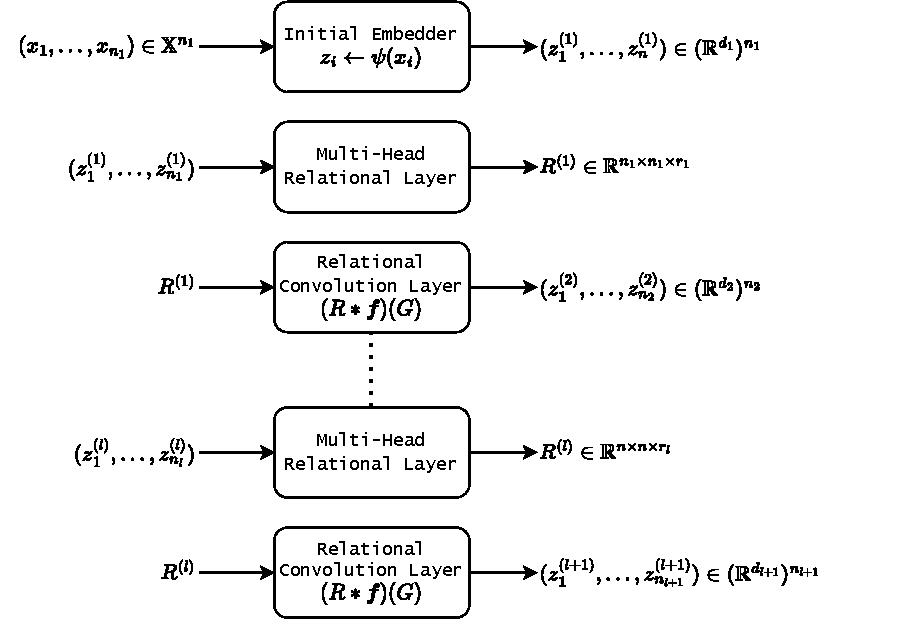
\includegraphics[width=0.75\textwidth]{figs/relational_framework.pdf}
%     \caption{A depiction of our proposed framework for hierarchical relational machine learning. At each layer, the multi-head relation module takes a sequence of objects as input and produces a relation tensor representing the relations between each pair of objects. The relational convolution layer then transforms the relation tensor into a sequence of objects each describing the relations within some group of objects at the previous layer. The next layer receives this sequence of objects as input and again models the relations within it. Thus, each layer computes relational features of a higher-order (i.e., relations on relations). \textit{Legend}: $d_l$ represents the dimension of the objects at layer $l$; $z_i^{(l)}$ is the $i$th object at the $l$th layer; $R^{(k)}$ is the relation tensor at layer $l$; $r_l$ is the dimension of the relations at layer $l$; $n_l$ is the number of objects at layer $l$.}\label{fig:relational_framework}
% \end{figure}


\begin{figure}[!ht]
    \centering
    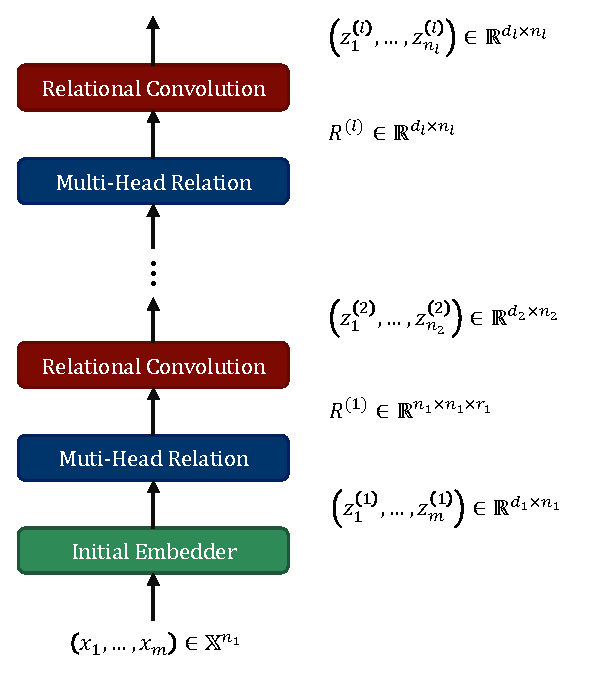
\includegraphics[width=.5\textwidth]{figs/relconv_architecture.pdf}
    \caption{Proposed framework for hierarchical relational machine learning. At each layer, the multi-head relation module takes a sequence of objects as input and produces a relation tensor representing the relations between each pair of objects. The relational convolution layer then transforms the relation tensor into a sequence of objects each describing the relations within some group of objects at the previous layer. The next layer receives this sequence of objects as input and again models the relations within it. Thus, each layer computes relational features of a higher order (i.e., relations on relations). \textit{Legend}: $d_l$ represents the dimension of the objects at layer $l$; $z_i^{(l)}$ is the $i$th object at the $l$th layer; $R^{(k)}$ is the relation tensor at layer $l$; $r_l$ is the dimension of the relations at layer $l$; $n_l$ is the number of objects at layer $l$.}\label{fig:relconv_architecture}
\end{figure}